% !Mode:: "TeX:UTF-8"
\section{可动边界的变分问题}
\subsection{最简泛函的变分问题}
设泛函
\begin{equation}
  J[y(x)]=\int_{x_0}^{x_1}F(x,y,y')dx
\label{equation.function.simple-general}
\end{equation}

其可取曲线$y = y(x) \in C^2$类函数,且两个端点$A(x_0,y_0),B(x_1,y_1)$ 分别在两个给定的$C^2$类函数,此时称为可动边界的最简泛函或待定边界的最简泛函。\\

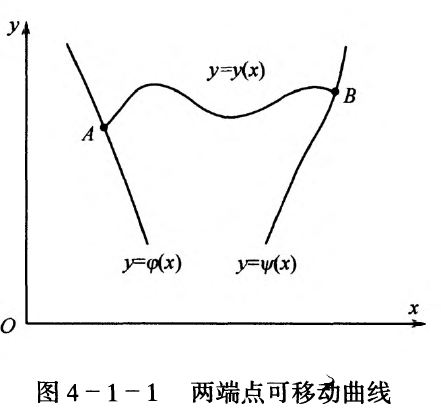
\includegraphics[width=0.5\textwidth]{image/limit-move}\\

若函数$y=y(x)$能在可动边界的容许函数类中使泛函(\ref{equation.function.simple-general})取得极值,
那么必能在固定边界的容许函数类中使泛函取得极值,这是因为可动边界泛函的容许曲线类的范围扩大了,当然包含了固定边界泛函的容许曲线,
而在固定边界情况下使泛函取得极值的函数必须满足欧拉方程,所以函数(\ref{equation.function.simple-general})在可动边界情况下也应当满足欧拉方程
$$
F_y - \frac{d}{dx}F_{y'} =0
$$
欧拉方程的解含有两个任意常数,它的一般解形式为
$$y=y(x,c_1,c_2)$$
在端点固定的情况下,这两个常数可以解出来,在可动边界条件下,他们都是$x_0,x_1$的函数,确定他们的条件就是泛函取得极值的必要条件$\delta J=0$

如图所示,A点固定,B点可以变动,当B点从$(x_1,y_1)$移动到$(x_1+\delta x_1,y_1+\delta y_1)$时,泛函$ J[y(x)]$的增量
\begin{equation}
     \begin{split}
         & \Delta J=\int_{x_0}^{x_1+\delta x_1}F(x,y+\delta y,y'+\delta y')dx-\int_{x_0}^{x_1}F(x,y,y')dx\\
         & =\int_{x_0}^{x_1+\delta x_1}F(x,y+\delta y,y'+\delta y')dx+\int_{x_0}^{x_1}[F(x,y+\delta y,y'+\delta y')-F(x,y,y')]dx
     \end{split}
\end{equation}
略去高阶无穷小量后剩下一阶变分为
\begin{equation}
\begin{split}
     &  \delta J=\int_{x_0}^{x_1}(F_y - \frac{d}{dx}F_{y'} )\delta y dx + F|_{x=x_1}\delta x_1 + F_{y'}|_{x=x_1}[\delta y_1 - y'(x_1)\delta x_1] \\
    & =\int_{x_0}^{x_1}(F_y - \frac{d}{dx}F_{y'} )\delta y dx + (F-y'F_{y'})|_{x=x_1}\delta x_1 +F_{y'}|_{x=x_1}\delta y_1
\end{split}
\end{equation}
因为泛函的极值只能在极值曲线上取得,所以
$F_y - \frac{d}{dx}F_{y'} \equiv0$
上式化为
\begin{equation}
     \delta J=(F-y'F_{y'})|_{x=x_1}\delta x_1 +F_{y'}|_{x=x_1}\delta y_1
\end{equation}
再由条件$\delta J=0$得
\begin{equation}
     (F-y'F_{y'})|_{x=x_1}\delta x_1 +F_{y'}|_{x=x_1}\delta y_1=0
     \label{equation.result.general}
\end{equation}
如果$\delta x_1,\delta y_1$相互无关,则由(\ref{equation.result.general})得到
\begin{equation}
(F-y'F_{y'})|_{x=x_1}=0
\label{equation.result.unrelated.1}
\end{equation}
\begin{equation}
F_{y'}=0
\label{equation.result.unrelated.2}
\end{equation}
当我们把(\ref{equation.result.unrelated.2})代入(\ref{equation.result.unrelated.1})我们得到$F_y=0$,因此我们有必要考虑$\delta x_1,\delta y_1$相关
\begin{theorem}
设泛函$J[y(x)]=\int_{x_0}^{x_1}F(x,y,y')dx$的极值曲线$y=y(x)$一端固定,另一端在直线$x=x_1$上待定,则可动的一端必满足自然边界条件(\ref{equation.result.unrelated.2})
若极值曲线$y=y(x)$的端点在已知直线$y=\psi(x)$上待定,则变分$\delta x_1,\delta y_1$相关
\end{theorem}

\begin{theorem}
设泛函$J[y(x)]=\int_{x_0}^{x_1}F(x,y,y')dx$的极值曲线$y=y(x)$左端固定,右端点在已知直线$y=\psi(x)$上待定,则右端点在$x=x_1$处必满足
\begin{equation}
[F + (\psi' - y')F_{y'}]|_{x=x_1}=0
\end{equation}
\end{theorem}
\begin{proof}
 对已知曲线$y=\psi(x)$取变分,得到 $\delta y=\psi'(x)\delta x$,在右端点处,$\delta y_1=\psi'(x_1)\delta x_1$ \\
将之代入到(\ref{equation.result.general})可以得到
$$
[F + (\psi' - y')F_{y'}]|_{x=x_1}\delta x_1=0
$$
又因为$\delta x_1$是任意的,所以可以得到
$[F + (\psi' - y')F_{y'}]|_{x=x_1}=0$
\end{proof}
上式建立了极值曲线$y = y ( x )$与已知曲线:$y = \psi(x)$在交点B 处的$y'$与$\psi'$两斜率
之间的关系,这样的关系称为横截(性)条件、贯截条件或斜截条件。这两条曲线较小的那个交角称
为斜截角。

\begin{theorem}
\label{theorem.limit.two}
设泛函$J[y(x)]=\int_{x_0}^{x_1}F(x,y,y')dx$的极值曲线$y=y(x)$左端固定在直线$y=\varphi(x)$,右端点在已知直线$y=\psi(x)$上待定,\\
则左端点在$x=x_0$处必满足
\begin{equation}
[F + (\varphi' - y')F_{y'}]|_{x=x_0}=0
\end{equation}
则右端点在$x=x_1$处必满足
\begin{equation}
[F + (\psi' - y')F_{y'}]|_{x=x_1}=0
\end{equation}
\end{theorem}
求平面上两条曲线的最短距离是定理(\ref{theorem.limit.two})的一个常见的应用,在此情况下,该定理可以化为更具体的形式.该问题归结为求泛函
$$J[y]=\int_{x_0}^{x_1}\sqrt{1+y'^2}dx$$的极小值

\subsection{含有多个函数的泛函的变分问题}
设空间曲线
\begin{equation}
J[y(x),z(x)]=\int_{x_0}^{x_1}F(x,y,z,y',z')dx
\label{equation.general.space}
\end{equation}
式中$y,z \in C^2[x_0,x_1],F \in C^2$,容许曲线$y=y(x),z=z(x)$在左端点
$A(x_0,y_0,z_0)$固定,右端点 $B(x_1,y_1,z_1)$待定
泛函的(\ref{equation.general.space})的变分可模仿上节的方法进行
\begin{equation}
\begin{array}{c}
  \Delta J=\int_{x_0}^{x_1+\delta x_1}F(x,y+\delta y,z+\delta z,y'+\delta y',z'+\delta z')dx-\int_{x_0}^{x_1}F(x,y,z,y',z')dx\\
\\
  = \int_{x_1}^{x_1+\delta x_1}F(x,y+\delta y,z+\delta z,y'+\delta y',z'+\delta z')dx +\\
\\
\int_{x_0}^{x_1}[F(x,y+\delta y,z+\delta z,y'+\delta y',z'+\delta z')-F(x,y,z,y',z')]dx
\end{array}
\end{equation}
它的线性主部
\begin{equation}
 \delta J=F|_{x=x_1}\delta x_1 +F_{y'}\delta y|_{x=x_1} +F_{z'}\delta z|_{x=x_1} +
 \int_{x_0}^{x_1}[(F_y - \frac{d}{dx}F_{y'}) \delta y +(F_z -\frac{d}{dx}F_{z'} )\delta z]dx
\end{equation}
因为泛函$J[y,z]$的极值只能在极值曲线上取得,故必须满足欧拉方程组
$$
\left\{
  \begin{array}{ll}
    F_y - \frac{d}{dx}F_{y'}=0 & \\
    F_z - \frac{d}{dx}F_{z'}=0 &
  \end{array}
\right.
$$
这个方程组的通解中含有四个任意常数,由于B点可以变动,又多了一个未知量$x_1$,为了使泛函(\ref{equation.general.space})有唯一一组解,就需要确定五个常数.因为A点固定,由$y(x_0)=y_0,z(x_0)=z_0$可以定出两个常数,其余三个常数可根据泛函的极值条件$\delta J=0$确定
将欧拉方程组代入得到
\begin{equation}
 \delta J=F|_{x=x_1}\delta x_1 +F_{y'}\delta y|_{x=x_1} +F_{z'}\delta z|_{x=x_1}=0
\end{equation}
根据上一节的讨论有
\begin{equation}
 \delta y|_{x=x_1}=\delta y_1 - y'(x_1)\delta x_1, \delta z|_{x=x_1}=\delta z_1 - z'(x_1)\delta x_1
\end{equation}
代入上式得
\begin{equation}
 \delta J=(F - y'F_{y'} - z'F_{z'})|_{x=x_1} + F_{y'}|_{x=x_1}\delta y_1 + F_{z'}|_{x=x_1}\delta z_1=0
\label{equation.cases}
\end{equation}
式中的$\delta x_1.\delta y_1,\delta z_1$是任意的,即B点可以按照任意方式变动.根据$y_1,z_1与x_1$之间的关系,可分四种情况来讨论
\\
(1)若变分$\delta x_1.\delta y_1,\delta z_1$相互无关,则可以得到
$$
\left\{
  \begin{array}{ll}
     & (F - y'F_{y'} - z'F_{z'})|_{x=x_1}=0 \\
     &  F_{y'}|_{x=x_1}=0\\
     & F_{z'}|_{x=x_1}=0
  \end{array}
\right.
$$
此时,如果把后两式代入第一个式子中,则有$F|_{x=x_1}=0$,即泛函的被积函数为零,一般来说这样的变分问题无意义
\\
(2)若边界点$B(x_1,y_1,z_1)$沿着某一曲线
$y_1=\varphi(x_1),z_1=\psi(x_1)$
变动时,则
$\delta y_1=\varphi'(x_1)\delta x_1,\delta z_1=\psi'(x_1)\delta x_1$
将他们代入(\ref{equation.cases})并整理,同时注意到$\delta x_1$是任意的,得
\begin{equation}
 [F + (\varphi' - y')F_{y'} + (\psi' -z')F_{z'}]|_{x=x_1}=0
\label{equation.case2}
\end{equation}
式(\ref{equation.case2})称为泛函$J[y,z]$的极值曲线与端点曲线及极值问题的横截条件,它与方程
$y_1=\varphi(x_1),z_1=\phi(x_1)$
一起就能确定欧拉方程组的通解中的任意常数
\\
(3)若边界点$B(x_1,y_1,z_1)$沿着某一曲面$\phi(x_1,y_1,z_1)=0$变动,则
\begin{equation}
 \phi_{x_1}\delta x_1+
 \phi_{y_1}\delta y_1+
 \phi_{z_1}\delta z_1=0
\end{equation}
设$\phi_{x_1}\neq 0$,则可解出$\delta z_1$
代入(\ref{equation.cases})得
\begin{equation}
(F - y'F_{y'} - z'F_{z'} - F_{z'}\frac{\phi_x}{\phi_z})|_{x=x_1} \delta x_1 +
(F_{z'} -F_{z'}\frac{\phi_y}{\phi_z})|_{x=x_1} \delta y_1  )
=0
\end{equation}
由于$\delta x_1,\delta y_1$是任意的,故边界条件为
\begin{equation}
\left\{
  \begin{array}{lll}
     & (F - y'F_{y'} - z'F_{z'} - F_{z'}\frac{\phi_x}{\phi_z})|_{x=x_1} =0 \\
&\\
    & (F_{z'} -F_{z'}\frac{\phi_y}{\phi_z})|_{x=x_1} =0
  \end{array}
\right.
\label{equation.case3}
\end{equation}
将(\ref{equation.case3})与曲面方程$\phi(x_1,y_1,z_1)=0$联立,即可求出极值曲线
\\
(4)若边界点$B(x_1,y_1,z_1)$可在空间平面$x=x_1$上变动,则$\delta x_1=0$,$\delta y_1,\delta z_1$可任意取值,自然边界条件为
\begin{equation}
F_{y'}|_{x=x_1}=0,
F_{z'}|_{x=x_1}=0
\end{equation}

\subsection{含有高阶导数的泛函的变分问题}
设泛函
\begin{equation}
 J[y(x)]=\int_{x_0}^{x_1}F(x,y,y',y'')dx
\end{equation}
式中$y \in C^2[x_0,x_1],F \in C^3$,容许曲线$y=y(x)$在左端点$A(x_0,y_0)$固定,在右端点$B(x_1,y_1)$可变,泛函的极值曲线必满足欧拉-泊松方程
$$F_y - \frac{d}{dx}F_{y'} + \frac{d^2}{dx^2}F_{y''}=0  $$
通常情况下,上式是一个四阶微分方程,其通解含有四个任意常数,右端点B可变,所以$x_1$也待定,总共五个任意常数,左端点A固定可以确定两个,
剩余的三个任意常数必须通过泛函取得极值的必要条件$\delta J=0$得到
这里还是就一般情况进行讨论,先计算泛函的增量$\Delta J$,然后再分离出线性主部$\delta J$
泛函的增量
\begin{equation}
 \begin{split}
 \Delta J = & \int_{x_0}^{x_1+\delta x_1}F(x,y+\delta y,y'+\delta y',y''+\delta y'')dx- \int_{x_0}^{x_1}F(x,y,y',y'')dx \\
              &  =\int_{x_1}^{x_1+\delta x_1}F(x,y+\delta y,y'+\delta y',y''+\delta y'')dx + \\
               & \int_{x_0}^{x_1}[F(x,y+\delta y,y'+\delta y',y''+\delta y'') -F(x,y,y',y'') ]dx
 \end{split}
\end{equation}
最后化简得
\begin{equation}
\begin{split}
 \delta J = & [F - y'(F_{y'}-\frac{d}{dx}F_{y''}) - y''F_{y''}]|_{x=x_1} \delta x_1 + \\
 & (F_{y'}-\frac{d}{dx}F_{y''})|_{x=x_1}\delta y_1 + F_{y''}\delta y_1 =0
\end{split}
\end{equation}
如果上式中$\delta x , \delta y_1, \delta y'_1$之间是相互独立的,则他们的系数在点$x=x_1$处应该为零,及自然边界条件
\begin{equation}
\left\{
  \begin{array}{ll}
[F - y'(F_{y'}-\frac{d}{dx}F_{y''}) - y''F_{y''}]|_{x=x_1}=0 \\
(F_{y'}-\frac{d}{dx}F_{y''})|_{x=x_1}=0\\
F_{y''}=0
  \end{array}
\right.
\end{equation}
同样,若把后两式代入第一式中,仍可得到$F|_{x=x_1}=0$,一般情况下,这样的变分问题无意义.若使变分问题有意义,应在可动的右端点给出一个已知条件。于
是,三个式子中的后两个条件、右端点给出的一个已知条件加上固定端点的两个条件,就可以确 定极值曲线
$y=y(x,c_1,c_2,c_3,c_4)$中的五个待定常量
中的五个待定常量。
\begin{theorem}
 高阶泛函在某一端点固定$y(x_0)=y_0,y'(x_0)=y'_0$,另一端点$(x_1,y_1)$在给定一个已知条件下,其极值曲线$y=y(x)$在端点处
必满足自然边界条件的后两个条件
\end{theorem}

\subsection{单侧变分问题}
如果变分问题中的极值函数服从于某个不等式,则把受有这种不等式约束的变分问题成为单侧变分问题.考虑最简泛函
\begin{equation}
 J[y(x)]=\int_{x_0}^{x_1}F(x,y,y')dx
\end{equation}
在不等式
\begin{equation}
 y(x) \geqslant \varphi(x)
\end{equation}
约束条件下的极值条件,其中$\varphi(x)$是给定的具有连续倒数的函数
\begin{theorem}
 极值曲线$y=y(x)$与曲线$y=\varphi(x)$在M,N两点相切
\end{theorem}
